\documentclass[10pt]{article}
%------------------------------------------------------
\def\BibTeX{{\rm B\kern-.05em{\sc i\kern-.025em b}\kern-.08em
    T\kern-.1667em\lower.7ex\hbox{E}\kern-.125emX}}
\newtheorem{theorem}{Theorem}
\setcounter{page}{1}
\usepackage[utf8]{inputenc}
\usepackage{dsfont}
\usepackage{eso-pic}
%\newcommand{\treq}[0]{\triangleq}
%\newcommand{\mean}[1]{\mathcal{E}\left\{ #1 \right\} }
\usepackage[T1]{fontenc}
\usepackage[scaled]{beramono}
\usepackage{color}
\usepackage{upquote}
\usepackage{xcolor}
\usepackage{listings}
\usepackage{caption}
%-------------------------
\usepackage{array}
\usepackage{epsfig}
%\usepackage{psfig}
\usepackage{cite}
\usepackage{amsfonts}
\usepackage{amsmath}
\usepackage{amssymb}
\usepackage{amsxtra}
\usepackage{varioref}
\usepackage{multicol}
\usepackage{float}
\usepackage{rotate}
\usepackage{color}
\usepackage{enumerate}

\usepackage[spanish]{babel}
%\usepackage[latin1]{inputenc}

% ABAC PACKAGES
\usepackage{graphicx}
\usepackage{lineno}
\usepackage{hyperref}

%\renewcommand{\baselinestretch}{1.5}

\newcommand{\ltr}[1]{\ensuremath{{\cal{L}}\left[#1\right]}} %Laplace transform
\newcommand{\matriz}[1]{\left[\begin{matrix}#1\end{matrix}\right]}
% Matrices
\newcommand{\matrizr}[1]{\left(\begin{matrix}#1\end{matrix}\right)}
\newcommand{\matrizsc}[1]{\begin{matrix}#1\end{matrix}}
% Matrices sin corchetes
%\newcommand{\findemo}{\vspace{-12mm}\begin{flushright}$\Box\Box\Box$\end{flushright}}

\newcommand{\corregir}[1]{ \cal{K}_{\varepsilon} \ly #1 \ry }

\newcommand{\bs}[1]{\boldsymbol{#1}}
\newcommand{\ep}[0]{\operatorname{ep}}
\newcommand{\bp}[0]{\operatorname{bp}}
\newcommand{\opt}[0]{\operatorname{opt}}
\newcommand{\aux}[0]{\operatorname{aux}}
\newcommand{\stat}[0]{\operatorname{stat}}
\newcommand{\implica}[0]{\Rightarrow}
\newcommand{\contraimplica}[0]{\Leftarrow}
\newcommand{\tq}[0]{\textrm{ such that }}
\newcommand{\barra}[1]{\overline{#1}}
\newcommand{\non}[0]{\nonumber }
\newcommand{\ine}[1]{\left[ #1 \right]_{\mathcal{H}_2^{\perp}}}
\newcommand{\inep}[1]{\left[ #1 \right]_{\perp}}
\newcommand{\esti}[1]{\left[ #1 \right]_{\infty}}
\newcommand{\est}[1]{\left[ #1 \right]_{\mathcal{H}_2}}
\newcommand{\es}[0]{\textrm{ }}
\newcommand{\norma}[1]{\left| \left| #1 \right| \right|}
\newcommand{\equivale}[0]{\Leftrightarrow}

%\newcommand{\arginf}[1]{}

%\newcommand{\sol}[1]{\operatorname{sol} \left\{ #1 \right\}  }

\newcommand{\adiag}[1]{\operatorname{adiag} \left\{ #1 \right\}  }
\newcommand{\diag}[1]{\operatorname{diag} \left\{ #1 \right\}  }
\newcommand{\diagn}[2]{\operatorname{diag} \left\{ #1 \right\}_{1,\cdots, #2}}
\newcommand{\struc}[1]{\operatorname{structure}\left\{ #1 \right\}  }
\newcommand{\traza}[1]{\operatorname{trace}\left\{ #1 \right\} }
\newcommand{\den}[1]{\operatorname{den}\left\{ #1 \right\} }
\newcommand{\num}[1]{\operatorname{num}\left\{ #1 \right\} }
\newcommand{\spart}[1]{\operatorname{sp}\left\{ #1 \right\} }
\newcommand{\grel}[1]{\operatorname{grel}\left\{ #1 \right\} }
\newcommand{\gr}[1]{\operatorname{gr}\left\{ #1 \right\} }
\newcommand{\mean}[1]{\mathcal{E}\left\{ #1 \right\} }
\newcommand{\meanaux}[1]{\mathbb{E}\left\{ #1 \right\} }
\newcommand{\meancr}[2]{\mathcal{E}_{#1}\left\{ #2 \right\} }
\newcommand{\abs}[1]{\left| #1 \right| }
\newcommand{\ejw}[0]{(e^{j\omega})}
\newcommand{\ejwo}[0]{(e^{j\omega_o})}
\newcommand{\ejws}[0]{e^{j\omega}}
\newcommand{\z}[0]{(z)}
\newcommand{\floor}[1]{ \left \lfloor #1 \right \rfloor}
\newcommand{\treq}[0]{\triangleq}
\newcommand{\normaex}[1]{\frac{1}{2\pi}\int_{-\pi}^{\pi} \abs{  #1  }^2 d\omega }
\newcommand{\intpi}[1]{\int_{-\pi}^{\pi} #1 d\omega }
\newcommand{\intpifrac}[1]{\frac{1}{2\pi}\int_{-\pi}^{\pi} #1 d\omega }
\newcommand{\intpifracK}[2]{\frac{#1 }{2\pi}\int_{-\pi}^{\pi} #2 d\omega }
\newcommand{\intbode}[1]{\frac{1}{2\pi}\int_{-\pi}^{\pi} \ln\lp #1 \rp d\omega }
\newcommand{\intbodeK}[2]{\frac{#1}{2\pi}\int_{-\pi}^{\pi} \ln\lp #2 \rp d\omega }
\newcommand{\intbodesin}[1]{\int_{-\pi}^{\pi} \ln\lp #1 \rp d\omega }
\newcommand{\intbodemod}[1]{\frac{1}{2\pi}\int_{-\pi}^{\pi} \ln #1 d\omega }
\newcommand{\intbodesinmod}[1]{\int_{-\pi}^{\pi} \ln #1  d\omega }
\newcommand{\normaexsinpi}[1]{\int_{-\pi}^{\pi} \abs{  #1  }^2 d\omega }

\newcommand{\evalinf}[1]{ \lpt \ly #1 \ry \right|_{z=\infty} }
\newcommand{\eval}[2]{ \lpt \ly #1 \ry \right|_{z=#2} }
\newcommand{\evalnoz}[3]{ \lpt \ly #1 \ry \right|_{#2=#3} }
\newcommand{\evalnoy}[3]{ \lpt #1 \right|_{#2=#3} }
\newcommand{\evalnoll}[3]{ \lpt #1 \right|_{#2=#3} }
\newcommand{\dado}[2]{ \lpt #1 \right|_{#2} }

\newcommand{\problemas}[1]{ \begin{pregunta} \emph{ #1 } \end{pregunta}}

\newcommand{\MSS}{\operatorname{MSS}}

\newcommand{\estimador}[2]{ \lpt \hat{#1} \right|_{#2} }

\newcommand{\sat}[2]{\text{\rm sat} \left ( #1 ,#2 \right ) }
\newcommand{\unif}[2]{\text{\rm Unif} \left (#1,#2\right)}

\newcommand{\nf}{\operatorname{nf}}

\renewcommand{\H}[0]{ \mathbb{H}}
\newcommand{\D}[0]{ \mathbb{D}}
\newcommand{\R}[0]{ \mathbb{R}}
\newcommand{\T}[0]{ \mathbb{T}}
\newcommand{\Q}[0]{ \mathbb{Q}}
\newcommand{\N}[0]{ \mathbb{N}}
\newcommand{\B}[0]{ \mathbb{B}}
\newcommand{\X}[0]{ \mathbb{X}}
\renewcommand{\P}[0]{ \mathbb{P}}
\newcommand{\U}[0]{ \mathbb{U}}
\newcommand{\Z}[0]{ \mathbb{Z}}
\newcommand{\C}[0]{ \mathbb{C}}
\newcommand{\prodin}[2]{ \left \langle \, #1, #2 \,\right \rangle }
\newcommand{\signo}[1]{ \operatorname{sign}\lp #1\rp }
\renewcommand{\cal}{\mathcal}
\newcommand{\trafozb}[1]{\sum_{k=-\infty}^{\infty}  #1 z^{-k} }
\newcommand{\trafoz}[1]{\sum_{k=0}^{\infty}  #1 z^{-k} }
\newcommand{\sumainf}[1]{\sum_{#1 =-\infty}^{\infty} }
\newcommand{\doscasos}[2]{\ly \begin{array}{l} #1 \\ #2 \end{array}
\rpt}
\newcommand{\doscasosTres}[3]{\ly \begin{array}{l} #1 \\ #2  \\ #3 \end{array}
\rpt}
\newcommand{\doscasosCuatro}[4]{\ly \begin{array}{l} #1 \\ #2  \\ #3  \\ #4 \end{array}
\rpt}
\newcommand{\casosdosxdos}[4]{\ly \begin{array}{ll} #1 & #2 \\ #3 & #4 \end{array}
\rpt}
\newcommand{\casostresxdos}[6]{\ly \begin{array}{ll} #1 & #2 \\ #3 & #4 \\ #5 & #6\end{array}
\rpt}
\newcommand{\casosM}[4]{\ly \begin{array}{ll} #1 & #2 \\ \\ #3 & #4 \end{array}
\rpt}
\newcommand{\casosd}[4]{\ly \begin{array}{ll} #1 & #2 \\ #3 & #4 \end{array}
\ry}
\newcommand{\Ginvdc}{G^{-1}(1)}
\newcommand{\sigmaf}{\vec{\sigma}}
\newcommand{\uf}{\vec{u}}
\newcommand{\yf}{\vec{y}}
\newcommand{\xf}{\vec{x}}
\renewcommand{\sf}{\vec{s}}
\newcommand{\uo}[0]{u_{opt}}
\newcommand{\sigmaq}[0]{\sigma_{\hspace{-0.5mm} q}}
\newcommand{\im}[1]{\operatorname{Im} \ly #1 \ry}

\newcommand{\referencia}[0]{\operatorname{ref}}

\newcommand{\igual}[1]{ \stackrel{_{(#1)}}{=} }
\newcommand{\menori}[1]{ \stackrel{_{(#1)}}{\leq} }
\newcommand{\mayori}[1]{ \stackrel{_{(#1)}}{\geq} }
\newcommand{\mayor}[1]{ \stackrel{_{(#1)}}{>} }
\newcommand{\menor}[1]{ \stackrel{_{(#1)}}{<} }
\newcommand{\equivalen}[1]{ \stackrel{_{(#1)}}{\equivale} }

\renewcommand{\det}[1]{ \operatorname{det}\lp #1 \rp}

\newcommand{\dechat}[0]{ \bar{\mathscr{D}} }
\newcommand{\enchat}[0]{ \bar{\mathscr{E}} }
\newcommand{\markov}[0]{ \leftrightarrow }
\newcommand{\tofrom}[0]{ \leftrightarrows }
\newcommand{\dec}[0]{ \mathscr{D} }
\newcommand{\enc}[0]{ \mathscr{E} }

\newcommand{\arginf}[1]{ \underset{#1}{\operatorname{arg\, inf} } \; }
\newcommand{\argmin}[1]{ \underset{#1}{\operatorname{arg\, min} } \; }

\newcommand{\intomega}[1]{ \frac{1}{2\pi}\int_{-\pi}^{\pi} #1 d\omega }
\newcommand{\intomegaK}[2]{ \frac{#1}{2\pi}\int_{-\pi}^{\pi} #2 d\omega }

\newcommand{\mndelta}[0]{ \lp -\frac{\Delta}{2}, \frac{\Delta}{2} \rp }
\newcommand{\prob}[1]{ \operatorname{P_r}\ly #1 \ry }

\newcommand{\LT}[1]{ \cal{L}\ly #1 \ry }

\newcommand{\iid}[0]{i.i.d. \hspace{-1.5mm}}
\renewcommand{\ae}[0]{a.e. \hspace{-1mm}}

\newcommand{\fn}{\operatorname{fn}}
\newcommand{\activa}{\operatorname{act}}
\newcommand{\FP}{\operatorname{FP}}
\newcommand{\total}{\operatorname{total}}

\def\qed{\relax\ifmmode\hskip2em \blacksquare \else\unskip\nobreak\hskip1em $\blacksquare$\fi}

\newcommand{\mihrule}[0]{ \vspace*{2mm} \hrule \vspace*{2mm} }

\newcommand{\EC}{\operatorname{EC}}
\newcommand{\ECED}{\operatorname{EC-ED}}

\newtheorem{solucion}{\textbf{Soluci\'on del Problema}}
\newtheorem{pregunta}{\textbf{Problema}}[section]

\newtheorem{assu}{\textbf{Suposición}}
\newtheorem{problema}{\textbf{Problema}}
\newtheorem{ejercicio}{\textbf{Ejercicio}}
\newtheorem{problem}{\textbf{Problema}}
\newtheorem{nota}{\textbf{Observación}}
\newtheorem{coro}{\textbf{Corolario}}
\newtheorem{propo}{\textbf{Proposition}}
\newtheorem{lema}{\textbf{Lema}}
\newtheorem{teorema}{\textbf{Teorema}}
\newtheorem{ejemplo}{\textbf{Ejemplo}}
\newtheorem{defi}{\textbf{Definición}}
\newtheorem{remark}{\textbf{Nota}}
%\newtheorem{claim}{\textbf{Claim}}
%\newtheorem{req}{\textbf{Requirement}}
%\newtheorem{constraint}{\textbf{Constraint}}
\newtheorem{procedure}{\textbf{Procedure}}
\newtheorem{property}{\textbf{Property}}
%\newtheorem{fact}{\textbf{Fact}}
\newtheorem{algoritmo}{\textbf{Algorithm}}

%\newcommand{\findemo}{\hfill{$\blacksquare$}} %\hspace*{\fill}~$\square\square\square$} %\hfill{$\Box\Box\Box$} \\ }
\newcommand{\finassu}{\hfill{$\Box\Box$} \\}
\newcommand{\finejem}{\hfill{$\Box$} \\}
\newcommand{\findef}{ $\Box$ }
\newcommand{\fin}{~$\blacksquare$}
\newcommand{\findemo}{\fin \bigskip}
\newcommand{\finM}{\hspace*{\fill}~\square\square}

\newcommand{\Perp}{\perp \! \! \! \perp}

%\def\QED{\hfill{\mbox{\rule[0pt]{1.3ex}{1.3ex}}}} % for a filled box

\def\proof{\noindent{\textbf{Demostración:} }}
\def\endproof{\par\endtrivlist}

\def\solucion{\noindent{\textbf{Solución:} }}
\def\endproof{\par\endtrivlist}


\newcommand{\indep}{\perp \! \! \! \perp}

\def\further{\bigskip \noindent{\textbf{Further reading and sources:} \bfseries }}
\def\endfurther{\bigskip}

% Colores

\newcommand {\fire}[1]{{\color[rgb]{0.6953, 0.1328, 0.1328} {#1}}}
\newcommand {\green}[1]{{\color[rgb]{0,0.3906,0} {#1}}}
\newcommand {\red}[1]{{\color[rgb]{1,0,0} {#1}}}
\newcommand {\white}[1]{{\color[rgb]{1,1,1} {#1}}}
\newcommand {\blue}[1]{{\color[rgb]{0,0,1} {#1}}}
\newcommand {\magenta}[1]{{\color[rgb]{1,0,1} {#1}}}

\newcommand{\Mbs}[1]{\ensuremath{\mathbf{#1}(s)}}
\newcommand{\Mbz}[1]{\ensuremath{\mathbf{#1}[z]}}
\newcommand{\Mbj}[1]{\ensuremath{\mathbf{#1}(j\omega)}}
\newcommand{\Mb}[1]{\ensuremath{\mathbf{#1}}}
%\newcommand{\jw}{j\omega}
\newcommand{\wn}{\omega _n}
\newcommand{\esd}{e^{s\Delta}}
\newcommand{\ejwd}{e^{j\omega \Delta}}

\newcommand{\inner}[1]{ \left\langle #1 \right\rangle }
\newcommand{\gen}[1]{ \operatorname{span}\ly #1 \ry }
\newcommand{\col}[1]{ \operatorname{col}\ly #1 \ry }

\newcommand{\vecK}[1]{ \mathrm{vec}\ly #1 \ry}
\newcommand{\reduce}{ \mathrm{red} }
\newcommand{\vecKi}[1]{ \mathrm{vec}^{-1} \ly #1 \ry}

\newcommand{\spec}[1]{ \mathrm{spec} \ly #1 \ry}

%\newcommand{\eq}{\triangleq}
\newcommand{\dw}{d\omega}

\renewcommand{\Im}[1]{ \operatorname{Im} \ly #1 \ry }
\renewcommand{\Re}[1]{ \operatorname{Re} \ly #1 \ry }


%================================================================================
% LO QUE SIGUE ERA DE DIEGO
%================================================================================
\newcommand{\rpt}{\right.}
\newcommand{\lpt}{\left.}
\newcommand{\lc}{\left[}
\newcommand{\ly}{\left\{}
\newcommand{\ry}{\right\}}
\newcommand{\rc}{\right]}
\newcommand{\lp}{\left(}
\newcommand{\rp}{\right)}

\newcommand{\ti}[1]{\ensuremath{\tilde{ #1 }}}
\newcommand{\ninf}[1]{\ensuremath{\left|\left| #1 \right|\right|_\infty}}
%\newcommand{\gr}[1]{\ensuremath{g_{r}\left\{#1\right\}}}
\newcommand{\HH}{\mathcal{H}_2}
\newcommand{\HHC}{\ensuremath{\mathcal{H}_2^{\perp}}}
\newcommand{\RHinf}{\ensuremath{\mathcal{RH}_\infty}}

\newcommand{\0}{\mathbf{0}}
\newcommand{\Ti}{\ensuremath{\mathcal{T}_i}}
\newcommand{\St}{\ensuremath{\mathcal{S}_t}}


\newcommand{\vectri}{\mathrm{vec_T}}

\newcommand{\SNR}{\text{SNR }}
\newcommand{\snr}{\text{signal-to-noise ratio}}
\newcommand{\Domega}{\Delta \omega}

\def\sqrtR{\mathpalette\DHLhksqrt}
\def\DHLhksqrt#1#2{\setbox0=\hbox{$#1\sqrt{#2\,}$}\dimen0=\ht0
\advance\dimen0-0.2\ht0
\setbox2=\hbox{\vrule height\ht0 depth -\dimen0}%
{\box0\lower0.4pt\box2}}


\newcommand{\iniciocomentario}{ \red{ \vspace{2mm} \hrule\vspace{2mm} } }
\newcommand{\fincomentario}{ \red{ \vspace{2mm} \hrule \vspace{2mm}} }

\newcommand{\derive}[2]{ \frac{\partial #1}{\partial #2}}

%

\allowdisplaybreaks

%\usepackage[bookmarks=true,bookmarksnumbered,colorlinks=true,linkcolor=black,citecolor=black,pdfstartview=FitV,linktocpage,dvipdfm]{hyperref}
%\usepackage[notcite, notref]{showkeys}

\addtolength{\textwidth}{40mm} \addtolength{\oddsidemargin}{-20mm}
\addtolength{\textheight}{30mm}\addtolength{\voffset}{-20mm}

%=============================================================================
\begin{document}

\hrule

\begin{center}
\Large \textbf{Herramientas para Estimación de Campos Receptivos (RF) desde Registros de Retina in vitro utilizando arreglo Multi Electrodo (MEA).
\\
Manual de Usuario y Referencia.}
\\
\normalsize Versión 4.2.\\
Aland Astudillo C., aland.astudillo.c@gmail.com \\
Departamento de Electrónica \\
Universidad Técnica Federico Santa María, Valparaíso, Chile. \\
 %N$^{\circ}$ 1 -- %Segundo Semestre de 2013 
(\today)
%\normalsize 10 de abril de 2013
\end{center}
\hrule \vspace{3mm}

% The paper headers
\markboth{ Estimación de Campos Receptivos - Manual de Usuario y Referencia, 2014}%
{A.Astudillo \MakeLowercase{}: Estimación de Campos Receptivos - Manual de Usuario y Referencia.}

Este manual sirve de guía para realizar el análisis de señales provenientes del registro de células ganglionares en retina utilizando Arreglo Multi Electrodo (Multi Electrode Array, MEA).  A partir del primer análisis se obtienen los spikes por unidad (neurona o célula hipotética), y además se realiza la obtención de la respectiva señal de sincronía con el estímulo. Utilizando los spikes de las unidades válidas, la señal de sincronía y el estímulo, se pueden estimar los campos receptivos (Receptive Fields, RF). A partir de los campos receptivos estimados se pueden estudiar sus curvas temporales y perfiles espacio - temporales, y por último realizar el ajuste gaussiano de cada campo receptivo obtenido. Utilizando toda esta información es posible realizar una caracterización funcional y espacial de las células encontradas.

\texttt{aland.astudillo.c@usm.cl}.
\\
\hrule \vspace{3mm}

\tableofcontents

\newpage

\section{ \textbf{DESCRIPCIÓN INICIAL} }

El resultado del registro MEA corresponde a un conjunto de archivos de datos de \textit{Multi Channel System} (\verb+*.mcd+) que contienen las señales resultantes para todos los canales de cada experimento. Es necesario tener claridad sobre el experimento realizado a través de la lectura de la bitácora (dada en formato digital o foto) generada en el experimento para poder determinar el archivo que será analizado. Para el caso de la estimación de campos receptivos se deben utilizar estímulos tipo checker board.

\section{ \textbf{INSTRUCCIONES} }

\subsection{ OBTENER LA SEÑAL DE SINCRONÍA }

Esta etapa se realiza en el programa Matlab. Desde el archivo \verb+*.mcd+ que se va a analizar se debe obtener la señal de sincronía, para ello se debe usar el script (\verb+*.m+) de Matlab \verb+get_synchrony_signal.m+. \\

Copiar el script \verb+*.m+ en la carpeta en donde se encuentra el archivo \verb+*.mcd+. Los parámetros que se deben modificar dentro de ese script son:
\begin{itemize}
\item pathname
\item filename
\item filename2 (realizar el cambio respectivo para usar sólo una variable en vez de dos)
\end{itemize} 

En \verb+pathname+ debe ir la ruta completa del lugar donde se encuentra el archivo \verb+*.mcd+, por ejemplo

\verb+pathname = 'C:\Users\ALIEN3\Desktop\resultados_26-12\';+ \\

En \verb+filename+ debe ir el nombre del archivo \verb+*.mcd+ (con la extensión incluida) del cual se desea extraer la señal de sincronía, por ejemplo

\verb+filename = 'datos0005.mcd';+ \\

En \verb+filename2+ va el nombre del archivo sin la extensión (parámetro eliminado para próxima versión), por ejemplo 

\verb+filename2 = 'datos0005';+ \\

Previo a la ejecución del script \verb+get_synchrony_signal.m+, se debe añadir al directorio de \textit{Matlab} la carpeta \textbf{"ns"}, la cual contiene las funciones de \textit{Neuroshare} para permitir leer archivos del tipo \verb+*.mcd+ desde \textit{Matlab} (o \textit{Python}). También se debe asegurar de tener en esa carpeta el archivo \verb+*.dll+ específico (librería de \textit{Neuroshare}) para el sistema operativo utilizado (caso de Sistema Operativo \textit{Windows}) o el archivo \verb+*.so+ (caso de \textit{Unix}). Existe una versión del \verb+get_synchrony_signal+ utilizado en \textit{Python} que puede realizar esta misma función para obtener la señal de sincronización (normalmente el canal 252 del archivo \verb+*.mcd+), pero no está documentada en esta guía. \\

Luego de añadir al path la carpeta \verb+ns+ y modificar los campos mencionados, se puede ejecutar el script \verb+get_synchrony_signal.m+ presionando F5 o con el botón Run. La salida del programa corresponde a un archivo \verb+*.mat+ con la señal de sincronía y una imagen de la señal en formato \verb+*.pdf+. El nombre del archivo de salida del script \verb+get_synchrony_signal.m+ quedará como 

\verb+syn_signal1_xxxxx.mat+, \\

donde la última porción del nombre \verb+xxxxx+ corresponde al mismo nombre definido como el parámetro \verb+filename2+. \\

\newpage

\subsection{ ANALIZAR LA SEÑAL DE SINCRONÍA }

Esta etapa se realiza en \textit{Matlab}. La señal obtenida en la etapa anterior es analizada en búsqueda de las posiciones exactas de cada frame en el tiempo. Se utiliza el archivo \verb+*.mat+ generado como \verb+syn_signal1_xxxxx.mat+, donde \verb+xxxxx+ corresponde al nombre del archivo \verb+*.mcd+ analizado, sin la extensión. El script para realizar lo descrito se llama \verb+sync_signal_analizer3.m+. \\

Se debe copiar este script en la carpeta en donde se encuentra el archivo \verb+*.mcd+ y donde se encuentra el archivo \verb+*.mat+ generado anteriormente. Los parámetros que se deben definir y cambiar en este script son \\

\verb+datosname+ \\

En \verb+datosname+ debe ir el nombre del archivo \verb+*.mcd+ (sin la extensión), por ejemplo \\

\verb+datosname = 'datos0005';+ \\

Ejecutar el script presionando F5 o el botón Run. Cuando se ejecute el script se mostrarán en pantalla los valores de promedio y desviación estándar de las distancias entre frames, en puntos. En este caso para 20kHz, e imágenes a 60Hz (frame rate), la distancia promedio entre frames es de 334 puntos y una desviación estándar de 2 puntos (aproximadamente). Si esto no se cumple, entonces quiere decir que existe un error en la detección de los tiempos de los frames en la señal de sincronización, y el análisis no se podrá hacer. Para corregir esto se debe cambiar el parámetro de búsqueda dentro de los ciclos de análisis de posiciones. \\

La salida del script corresponde a un archivo llamado  \\

\verb+inicio_fin_frame_xxxxx.txt+, \\

en donde \verb+xxxxx+ corresponde al nombre del archivo \verb+*.mcd+ analizado, determinado por el parámetro \verb+datosname+. Este archivo de texto contiene el tiempo de inicio y fin de cada frame, en puntos (en dos columnas). \\

\newpage

\subsection{ ANALIZAR DATOS DE REGISTRO: Ordenamiento de Espigas (SPIKE SORTING) }

Esta etapa se realiza utilizando \textit{Offline Sorter} (v3.3) de \textit{Plexon}, sólo disponible en sistema operativo \textit{Windows}. \\

La entrada corresponde al archivo \verb+*.mcd+ completo. Se recomienda que una vez cargado el archivo \verb+*.mcd+, este sea guardado y transformado a formato \textit{Plexon} \verb+*.plx+, lo cual permite trabajar de forma más rápida en la lectura de canales y la realización de todos los análisis de spike sorting realizados en \textit{Offline Sorter}.\\

El análisis consiste en 4 etapas: filtrado de la señal, detección de spikes, extracción de características (creación de sub espacio) y selección, y finalmente el clustering (agrupación en el sub espacio de caracteristicas creado). La primera etapa corresponde al filtrado de la señal (filtro pasa alto 100Hz Butterworth) en cada canal del multi electrodo (252 electrodos). La detección de los spikes (umbral inferior para detección de los spikes en su parte negativa) se realiza utilizando como medida umbral un factor que depende de la desviación estándar del ruido estimado o simplemente de un valor extraído desde la señal. Los spikes encontrados deben ser alineados o centrados y luego se realiza una extracción de características, utilizando Análisis de Componentes Principales (Principal Component Analysis, PCA). Finalmente se realiza una etapa de clustering (manual o automática, dependiendo del método seleccionado, entre los cuales existe K-Means, Valley Seek, T Distribution - Expectation Maximization, entre otros). El resultado corresponde a varios grupos o clústers, donde cada clúster equivale a una unidad o potencial célula a identificar. \\

El archivo resultante contendrá las señales continuas y además, los resultados de las unidades encontradas y sus respectivos tiempos de spikes. Existen varias opciones para realizar el guardado del archivo. Uno puede guardar el archivo completo o existe la opción de sólo guardar los spikes encontrados y sus respectivos tiempos. Una vez terminado el análisis, se guarda un archivo \verb+*.plx+, que contiene SÓLO los spikes y tiempos de spikes de las unidades celulares encontradas. El archivo \verb+*.plx+ debe ser nombrado como \\

\verb+xxxx_ts_fecha.plx+, \\

en donde \verb+xxxx+ corresponde al nombre del archivo \verb+*.mcd+ original, y fecha corresponde a la fecha del análisis, en formato dd-mm-aaaa. \\

%Nota: Algunas observaciones sobre el proceso de Spike Sorting son?(visualización a zoom de 30), identificación de spikes axónicos, etc .. otras observaciones \\

Nota: Existe una versión de Spike Sorting desarrollado localmente en \textit{Python}, denominado SSpy, pero esa versión no está documentada en esta guía. La implementación es funcional pero necesita una etapa de interfaz más potente y amistosa para poder realizar mejor las tareas necesarias de selección de grupos, etc. El código está disponible para su mejoramiento y utilización.\\

Nota: Existe una versión de Spike Sorting desarrollado localmente en \textit{Matlab}, denominado SSmat (símil de SSpy), pero no está documentado en esta guía. La implementación es funcional y escalable, pero falta una etapa de interfaz más amigable para realizar las selecciones de grupos de manera más amena. \\

\newpage

\subsection{ GUARDAR TIEMPOS DE SPIKES}
	
Utilizando el programa \textit{NeuroExplorer} (en \textit{Windows}), abrir el archivo \verb+*.plx+ guardado con los spikes y tiempos de spikes de las unidades obtenidas en la etapa anterior. Ir a la pestaña de \textbf{timestamps} y copiar toda la tabla de datos que aparece. Crear un archivo de texto nuevo (Block de notas, Notepad++) pegar los datos y guardar con extensión \verb+*.txt+. Guardar idealmente con el mismo nombre o similar a \verb+xxxx_timestamps_fecha.txt+, donde \verb+xxxx+ y \verb+fecha+ dependen del archivo de origen de este resultado (\verb+datos00xx+ y \verb+fecha+). \\

Abrir el script \verb+readwrite_timestamps_txt.py+ con un editor de texto. Editar los parámetros \verb+tsfolder+ y \verb+filetimestamps+. El parámetro \verb+tsfolder+ corresponde a la carpeta en donde se guardarán los tiempos de spike de cada unidad. Cada unidad tendrá sus tiempos de spikes en archivos de texto \verb+*.txt+ aislados, por ejemplo \\

\verb+tsfolder = 'TS_datos0003'+ \\

El segundo parámetro \verb+filetimestamps+ corresponde al nombre del archivo de texto en donde se guardaron los tiempos de spikes desde el archivo \verb+*.plx+ en el paso anterior \\

\verb+filetimestamps = 'xxxx_timestamps_fecha.plx'+ \\

donde \verb+xxxx+ y \verb+fecha+ dependen del archivo real revisado. Guardar los cambios y ejecutar desde command Windows (o desde terminal)\\

\verb+>> python readwrite_timestamps_txt.py+ \\

Se creará la carpeta respectiva (según el nombre definido por el parámetro tsfolder) y dentro se crearán los archivos \verb+*.txt+ para cada unidad o célula hipotética.\\

\newpage
% ------------------------------------
\subsection{ SPIKE TRIGGERED AVERAGE (STA) }

El Spike Triggered Average (STA) corresponde a la estimación lineal de los campos receptivos celulares utilizando los tiempos de disparo de las unidades de células y el estímulo que gatillo cada disparo. El STA más básico logra una representación lineal del campo receptivo, y corresponde a una descripción estadística promedio de todos los posibles estímulos que pueden gatillar disparo para una célula específica. \\

Para realizar el STA se pueden utilizar dos opciones. La primera opción es usar un código para realizar el STA para sólo una unidad específica. La segunda forma es utilizar un segundo código para realizar el STA a un conjunto de varias unidades analizando de manera consecutiva.  \\

% ------------------------------------
\subsubsection{ STA INDIVIDUAL: stapy}
	
Para utilizar la primera forma, mediante la cual se analiza sólo una unidad seleccionada arbitrariamente, se utiliza el script 
\verb+sta_v4_sspy_xxxx.py+, 
en donde xxxx debe ser reemplazado por el nombre del archivo \verb+*.mcd+ analizado, sin la extensión \verb+*.mcd+. Copiar el script \verb+sta_v4_sspy_xxxx+.py en la carpeta en donde se encuentre la carpeta \verb+tsfolder+, y el archivo \verb+inicio_fin_frame_xxxx.txt+. Además, es necesario conocer el lugar en donde se encuentra la carpeta contenedora de las imágenes (estímulos, imágenes \verb+*.png+ o \verb+*.jpg+ guardadas según índice). En este ejemplo la carpeta contenedora de las imágenes es denominada \verb+checkImages+.\\

La primera vez que se realiza el STA, se pueden hacer un par de pruebas de lectura de archivos (opcionalmente). Sin embargo, la primera vez se deben obtener la imagen promedio (\verb+mean_image.mat+) y generar un archivo que contiene los nombres de las direcciones de todas las imágenes (\verb+image_filenames.mat+ y \verb+image_filenames.txt+). \\

Abrir el archivo script y editar los siguientes parámetros \\
\begin{itemize}

\item \verb+stafolder+ : corresponde a la carpeta que contendrá los resultados del STA, por ejemplo \\

\verb+stafolder = 'STA_datos0003'+ \\

\item \verb+imageruta+ : corresponde a la ruta o path en donde se encuentra la carpeta que contiene las imágenes o estímulos, por ejemplo \\

\verb+imageruta = 'D:/'+ \\

\item \verb+imagefolder+ : corresponde al nombre de la carpeta contenedora de imágenes, por ejemplo \\

\verb+imagefolder = 'checkImages'+ \\

\item \verb+imagefiltro+ : corresponde al tipo o extensión de las imágenes que serán cargadas, por ejemplo \\

\verb+imagefiltro = '*.png'+\\

\item \verb+timefolder+ : corresponde al nombre de la carpeta que contiene las unidades y sus respectivos timestamps, por ejemplo  \\

\verb+timefolder = 'TS_datos0003/'+ \\

\item \verb+samplingRate+ : corresponde a la tasa de muestreo en Hz de los datos adquiridos originalmente, por ejemplo \\

\verb+samplingRate = 20000+ \\

\item \verb+numberframes+ : corresponde al número de frames antes del spike que serán utilizados para obtener el STA, por ejemplo \\

\verb+numberframes = 13+ \\

\item \verb+numberframespost+ : corresponde al número de frames después del spike que serán utilizados para calcular el STA, por ejemplo \\

\verb+numberframespost = 5+\\

\item \verb+synchronyfile+ : corresponde al nombre del archivo de texto que contiene los índices de tiempos de los frames, y que es el resultado del análisis de la señal de sincronía, visto en una de las etapas previas de este manual, por ejemplo \\

\verb+synchronyfile = 'inicio_fin_frame_datos0003.txt'+ \\

\item \verb+sizex+  : corresponde al tamaño en el eje x de la imagen a cargar, en pixeles, por ejemplo \\

\verb+sizex = 380+ \\

\item \verb+sizey+  : corresponde al tamaño en el eje y de la imagen a cargar, en pixeles, por ejemplo \\

\verb+sizey = 380+ \\

\item \verb+dolog+ : corresponde a la opción de guardar los resultados del STA escalados usando logaritmo (no utilizado, próxima versión estará obsoleto) , por ejemplo  \\

\verb+dolog = 0+ \\
\end{itemize}

Una vez editados estos parámetros, guardar los cambios y ejecutar desde command Windows (o terminal). El script necesita 5 parámetros de entrada: \\
\begin{itemize}
\item \verb+getimagenames+ : se utiliza la primera vez como parámetro activo para generar el archivo con la lista de los nombres y path de las imágenes. \\
\item \verb+openimagesandwrite+ : corresponde a un test para leer y escribir imágenes usando el paquete respectivo (opcional). \\
\item \verb+calculatemeanrf+ : se utiliza la primera vez como parámetro activo para calcular el estímulo promedio desde todas las imágenes.\\
\item \verb+tipoalgoritmo+ : corresponde al tipo de algoritmo a utilizar (cargar conjunto de imágenes completo o realizar una carga secuencial). El tipo de algoritmo utilizado actualmente corresponde al 2, ya que el primero está obsoleto momentáneamente.\\
\item \verb+timestampName+ : corresponde al nombre de la unidad a analizar, por ejemplo si la unidad a analizar corresponde a "C12a", se ingresa esa palabra. \\
\end{itemize}

Para ejecutar el código por primera vez para analizar la unidad C12a se escribe en command windows o en terminal \\
\verb+>> python sta_v4_sspy_xxxx.py 1 1 1 2 C12a+ \\
Luego de que se cumplan todas las etapas, se creará una carpeta denominada C12a dentro de la carpeta de STA (según el nombre definido como parámetro) que contendrá un número de frames y el promedio de esos frames. Además, la matriz STA y otros parámetros estarán guardados como archivos \verb+*.mat+. Cuando la unidad efectivamente corresponde a una célula, la dinámica espacio temporal del campo receptivo podrá ser visualizada en los diferentes frames resultantes.\\

Para ejecutar el código, luego para cualquier otra unidad, se puede escribir \\
\verb+>> python sta_v4_sspy_xxxx.py 0 0 0 2 G8a+ \\

Los parámetros iniciales ya no son necesarios, ya que tanto el archivo de imagen promedio (\verb+mean_image.mat+) y el archivo con la lista de imágenes (\verb+image_filenames.txt+) ya fueron creados.
Cada vez que se realice el análisis en un computador se debe crear una sola vez estos archivos. Si para varios análisis de STA de diferentes fechas las imágenes son las mismas utilizadas (es decir que la semilla para generar el checkerboard es la misma) es posible saltarse el paso de obtener la imagen promedio y la ruta de todas las imágenes, y saltar al paso de realizar el STA sin ningún problema. Sin embargo, se debe considerar siempre que para distintas fechas de análisis (un archivo de uno u otro experimento) se tendrán señales de sincronía distintas. Por lo tanto, el análisis de la señal de sincronía no es opcional, y se debe realizar siempre para cada archivo analizado.\\

Los archivos de salida que genera el script STA estarán contenidos en la carpeta STA definida por parámetro. Dentro de la carpeta estarán las carpetas de unidades, cuyos nombres son los respectivos a cada unidad analizada. Dentro de cada carpeta para cada unidad se encontrará la colección de frames en formato \verb+*.png+ correspondientes a la estimación del campo receptivo en una representación espacio temporal (ver figura \ref{fig:staframes}), el STA promedio, y archivos \verb+*.mat+ que contienen la matriz STA escalada para visualización y la matriz STA sin escalar; otro archivo \verb+*.mat+ conteniendo cada timestamp e índice de frame respectivo (para verificación). Los archivos se denominan \verb+stavisual_lin_array_xxxx.mat+ y \verb+spikeframe_matrixxxxx.mat+, respectivamente, donde \verb+xxxx+ corresponde al nombre de la unidad analizada.\\

\begin{center}
\begin{figure}[h!]
\centering
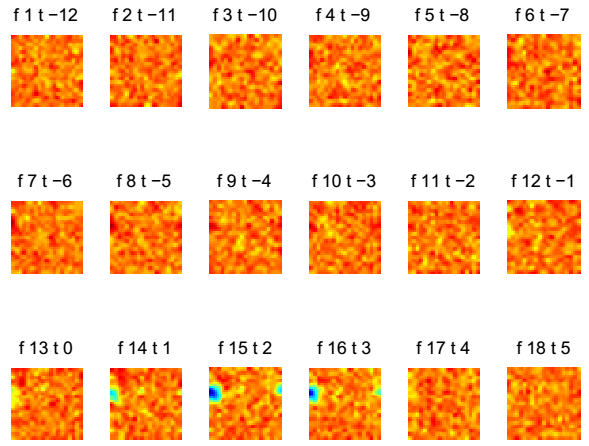
\includegraphics[scale=0.5, natwidth=640, natheight=480]{staframesraw_2.png} 	%{h_2.png}	\\				
\caption{ Colección de frames del STA obtenido para una unidad en particular. En este caso es posible decir que efectivamente aparece un campo receptivo. }
\label{fig:staframes}
\end{figure}
\end{center}

Nota: El tiempo de cálculo de un STA dependerá, entre otros, de la cantidad de spikes que tiene la unidad analizada. En promedio, un análisis de este tipo para una unidad que tiene 1000 spikes, puede tomar entre 10 a 15 minutos (Intel I7 2.GHz 8GB RAM, Windows7). \\

Nota: Existe una versión del STA actual que mejora la eficiencia del código. En lugar de leer las imágenes desde un directorio, carga un archivo \verb+*.mat+ con el estímulo comprimido a su tamaño original. Esto permite mejorar enormemente la eficiencia, disminuyendo el tiempo requerido para cada análisis. Esta versión estará disponible pronto.

Nota: La versión actual está siendo modificada para hacer más ameno el ingreso de variables y la definición de parámetros opcionales. 

% ------------------------------------
\subsubsection{ STA GRUPAL: stapy chain } 
	
Para ejecutar el análisis STA de un bloque o conjunto de unidades se debe usar el script \verb+sta_chain2_xxxx.py+ (se debe tener en la misma carpeta el archivo \verb+sta_functions2.py+), donde \verb+xxxx+ es reemplazado por el nombre del archivo \verb+*.mcd+ analizado. 
Copiar y pegar el script \verb+sta_chain2_xxxx.py+ en la misma carpeta en donde se encuentra la carpeta que contiene los resultados, en este ejemplo la carpeta se llama \verb+TS_datos0003+, por lo tanto los tiempos de disparo provienen del análisis del archivo denominado \verb+datos0003.mcd+, y por lo tanto el script queda como \verb+sta_chain2_datos0003.py+. Editar el script y modificar los siguientes parámetros \\

\begin{itemize}
\item \verb+archivosruta+ : corresponde a la ruta completa de donde se encuentra la carpeta que contiene los timestamps aislados en archivos \verb+*.txt+, por ejemplo\\

\verb+archivosruta = 'D:/Experimentos_CINV/datos_20-11-2013_bga50um_2/'+ \\

\item \verb+archivosfolder+ : corresponde al nombre de la carpeta que contiene los timestamps de las unidades a analizar, por ejemplo \\

\verb+archivosfolder = 'TS_datos0003/'+ \\

\item \verb+archivofiltro+ : corresponde a la extensión de los archivos que contienen los tiempos de spike (timestamps) de las unidades, y que funciona como filtro para cargar los archivos, en este caso se utiliza por defecto \\

\verb+archivofiltro = '*.txt'+ \\
\end{itemize}

Los parámetros \verb+getimagenames+, \verb+openimagesandwrite+, \verb+calculatemeanrf+ y \verb+tipoalgoritmo+ corresponden a los mismos definidos en el caso anterior y si no es primera vez que se ejecuta el código se pueden dejar como \\
\begin{itemize}
\item \verb+getimagenames = 0+
\item \verb+openimagesandwrite = 0+
\item \verb+calculatemeanrf = 0 +
\item \verb+tipoalgoritmo = 2+
\end{itemize}

Los siguientes parámetros son similares a los definidos en el caso anterior, y se pueden dejar, por ejemplo \\
\begin{itemize}
\item \verb+stafolder = 'STA_datos0003_2'+
\item \verb+imageruta = 'D:/'+
\item \verb+imagefolder = 'checkImages'+
\item \verb+imagefiltro = '*.png'+
\item \verb+samplingRate = 20000 +
\item \verb+numberframes = 18+
\item \verb+numberframespost = 2+
\item \verb+synchronyfile = 'inicio_fin_frame_datos0003.txt'+
\item \verb+sizex = 380 +
\item \verb+sizey = 380 +
\item \verb+dolog = 0+
\end{itemize}

Los últimos parámetros que se editan son inicio y final, con los cuales se define el intervalo de índices de las unidades que serán analizadas. Para saber el índice de una unidad, se debe tener en paralelo una tabla Excel en donde se ordenan las unidades con sus nombres e índices (recomendado). Estos parámetros pueden quedar, por ejemplo \\
\verb+inicio = 10 -1+ \\
\verb+final  = inicio - - 5+ \\
lo cual significa que se analizará desde la unidad 10 hasta la unidad 10+5, es decir 5 unidades, cuyos nombres se pueden ver en la tabla Excel según su índice. Al guardar los cambios y ejecutar, se obtendrá la creación de las carpetas respectivas y el análisis de cada unidad.\\

Nota: El script \verb+sta_chain2_xxxx.py+ utiliza al script \verb+sta_functions2.py+. Este script se ha modificado para permitir guardar la matriz STA real (cuyas amplitudes no han sido reescaladas, y es la que sirve ) y la matriz STA re escalada para visualización. Esto no sucede así en el caso del script que analiza las unidades de manera individual, pero para la siguiente versión si estará incluido para ambos casos. \\

Nota: Existe un formato para la generación de la tabla Excel que agrupa y ordena los resultados que se van obteniendo en cada uno de los análisis, y que además contiene el resultado del análisis por inspección de los campos receptivos obtenidos. Si bien este análisis es subjetivo, puede apoyarse por otros tipos de análisis para determinar si efectivamente el resultado del proceso de STA resulta en un campo receptivo real o no, y sirve como apoyo para los próximos pasos en el análisis. \\

% ------------------------------------
\subsubsection{ STA Rápido: stapy FAST } 

Usando una versión reducida del conjunto de estímulo, y en lugar de las imagenes en tamaño normal de presentación (380x380px), usar un archivo que contiene todos los frames en una resolución menor, sin perder las características que se pueden observar (es decir que la forma de cada bloque del checkerboard permanezca intacta, es posible obtener una versión del STA que demora mucho menos en el cálculo. \\

Para ejecutar el análisis STA de un bloque o conjunto de unidades se debe usar el script \verb+STA_FAST.py+. 
Copiar y pegar el script \verb+STA_FAST.py+ en la misma carpeta en donde se encuentra la carpeta que contiene los resultados del ordenamiento de spikes, en este ejemplo la carpeta se llama \verb+TS_datos0003+, por lo tanto los tiempos de disparo provienen del análisis del archivo denominado \verb+datos0003.mcd+. Los parámetros de entrada son los siguientes:\\

\begin{itemize}
\item \verb+archivosruta+ : corresponde a la ruta completa de donde se encuentra la carpeta que contiene los time stamps aislados en archivos \verb+*.txt+, por ejemplo\\

\verb+archivosruta = 'D:/Experimentos_CINV/datos_20-11-2013_bga50um_2/'+ \\

\item \verb+archivosfolder+ : corresponde al nombre de la carpeta que contiene los time stamps de las unidades a analizar, por ejemplo \\

\verb+archivosfolder = 'TS_datos0003/'+ \\

\item \verb+archivofiltro+ : corresponde a la extensión de los archivos que contienen los tiempos de spike (timestamps) de las unidades, y que funciona como filtro para cargar los archivos, en este caso se utiliza por defecto \\

\verb+archivofiltro = '*.txt'+ \\

\item \verb+getimagenames+ : corresponde a la realización de una carga de imágenes como prueba del paquete específico (en la próxima versión estará obsoleto). En este caso se deja como \\

 \verb+getimagenames = 0+ \\

\item \verb+openimagesandwrite+ : corresponde a una prueba del módulo (en la próxima versión estará obsoleto). En este caso se deja como \\

\verb+openimagesandwrite = 0+ \\

\item \verb+calculatemeanrf+ : corresponde al cálculo del estímulo medio, sólo para el caso en que se cargan las imágenes desde una carpeta contenedora (en la próxima versión estará obsoleto). Para este caso se deja como \\

\verb+calculatemeanrf = 0 + \\

\item \verb+tipoalgoritmo+ : corresponde al tipo de algoritmo a utilizar para calcular el STA. En este caso se utiliza el algoritmo tipo 4, para cargar un conjunto estímulo en un archivo \verb+*.mat+ \\

\verb+tipoalgoritmo = 4+ \\

\item \verb+stafolder+ : corresponde a la carpeta que contendrá los resultados del STA, por ejemplo \\

\verb+stafolder = 'STA_datos0003'+ \\

\item \verb+imageruta+ : corresponde a la ruta o path en donde se encuentra la carpeta que contiene las imágenes o estímulos, por ejemplo \\

\verb+imageruta = 'D:/'+ \\

\item \verb+imagefolder+ : corresponde al nombre de la carpeta contenedora de imágenes, por ejemplo \\

\verb+imagefolder = 'checkImages'+ \\

\item \verb+imagefiltro+ : corresponde al tipo o extensión de las imágenes que serán cargadas, por ejemplo \\

\verb+imagefiltro = '*.png'+\\

\item \verb+timefolder+ : corresponde al nombre de la carpeta que contiene las unidades y sus respectivos timestamps, por ejemplo  \\

\verb+timefolder = 'TS_datos0003/'+ \\

\item \verb+samplingRate+ : corresponde a la tasa de muestreo en Hz de los datos adquiridos originalmente, por ejemplo \\

\verb+samplingRate = 20000+ \\

\item \verb+numberframes+ : corresponde al número de frames antes del spike que serán utilizados para obtener el STA, por ejemplo \\

\verb+numberframes = 13+ \\

\item \verb+numberframespost+ : corresponde al número de frames después del spike que serán utilizados para calcular el STA, por ejemplo \\

\verb+numberframespost = 5+\\

\item \verb+synchronyfile+ : corresponde al nombre del archivo de texto que contiene los índices de tiempos de los frames, y que es el resultado del análisis de la señal de sincronía, visto en una de las etapas previas de este manual, por ejemplo \\

\verb+synchronyfile = 'inicio_fin_frame_datos0003.txt'+ \\

\item \verb+sizex+  : corresponde al tamaño en el eje x de la imagen a cargar, en pixeles, por ejemplo \\

\verb+sizex = 380+ \\

\item \verb+sizey+  : corresponde al tamaño en el eje y de la imagen a cargar, en pixeles, por ejemplo \\

\verb+sizey = 380+ \\

\item \verb+dolog+ : corresponde a la opción de guardar los resultados del STA escalados usando logaritmo (no utilizado, en la próxima versión estará obsoleto) , definir como  \\

\verb+dolog = 0+ \\

\item \verb+stim_mini+ : corresponde al nombre del archivo \verb+*.mat+ que contiene el conjunto de estímulos en una versión reducida. En este caso dejar como \\

\verb+ stim_mini = stim_mini.mat+ \\

\end{itemize}

Los últimos parámetros que se editan son inicio y final, con los cuales se define el intervalo de índices de las unidades que serán analizadas. Para saber el índice de una unidad, se recomienda contar con un archivo Excel en donde se pueda revisar en paralelo las unidades con sus nombres y números. Los parámetros de inicio y fin pueden quedar, por ejemplo \\
\verb+inicio = 10 -1+ \\
\verb+final  = inicio - - 5+ \\
lo cual significa que se analizará desde la unidad 10 hasta la unidad 10+5, es decir 5 unidades, cuyos nombres se podrían ver en la tabla Excel según su índice. Al guardar los cambios y ejecutar, se obtendrá la creación de las carpetas respectivas y el análisis de cada unidad.\\

Nota: Este script contiene las modificaciones respectivas para cargar el conjunto de estímulos desde un archivo mat. Además, se ha modificado para permitir guardar la matriz STA real (cuyas amplitudes no han sido re escaladas para el análisis) y la matriz STA re escalada para visualización. \\

Nota: Existe un formato para la generación de la tabla Excel que agrupa y ordena los resultados que se van obteniendo en cada uno de los análisis, y que además contiene el resultado del análisis por inspección de los campos receptivos obtenidos. Si bien este análisis es subjetivo, puede apoyarse por otros tipos de análisis para determinar si efectivamente el resultado del proceso de STA resulta en un campo receptivo real o no, y sirve como apoyo para los próximos pasos en el análisis. \\

Nota: Es posible que esta versión reemplace finalmente a las dos versiones anteriores debido al menor costo en cálculos y tiempo que requiere. Por esta razón, en la próxima versión del manual ya no se incluirán stapy ni stapy chain.

\newpage

% ------------------------------------
\subsection{ VALORIZACIÓN DE LOS CAMPOS RECEPTIVOS ESTIMADOS }

No siempre ocurre que se obtienen campos receptivos verdaderos cuando se analiza un tren de spikes y el estímulo respectivo. Por lo tanto, es necesario revisar cada resultado para cada tren de spikes e inspeccionar y declarar si efectivamente cada archivo resultante corresponde o no a un campo receptivo real y perceptible. Como esta tarea de inspección de campos receptivos es subjetiva, es necesario contar con una valorización objetiva que simplifique la tarea de inspección, y facilite esta tarea. Por este motivo se tiene el código \verb+sta_inspector.m+, el cual arroja un valor porcentual de calidad de STA realizado en función de los valores peak y variaciones de cada frame del STA.\\

Los parámetros de este script son

\verb+sta_folder+ : corresponde al nombre de la carpeta que contiene los resultados del STA, por ejemplo \\

\verb+sta_folder= 'STA_datos0003_2/';+ \\

\verb+ts_folder+ : corresponde al nombre de la carpeta que contiene los archivos de  time stamps, por ejemplo \\

\verb+ts_folder= 'TS_datos003_2/'];+ \\

El script analizará todos los archivos contenidos de matriz de campo receptivo estimado resultantes del STA y arrojará un vector en donde valoriza la calidad de cada STA. Aquellos STA con valores bajo cierto umbral, no corresponderán a un campo receptivo perceptible, por lo tanto sólo se inspeccionan aquellos STA que si cumplen con el umbral.

\newpage

% ------------------------------------
\subsection{ REALIZAR AJUSTE GAUSSIANO DE LOS CAMPOS RECEPTIVOS }

Para cada STA de las unidades analizadas en los pasos anteriores, es posible realizar el ajuste gaussiano y análisis de su dinámica temporal, con el objetivo de caracterizar tanto temporal como espacialmente (tamaño) cada unidad o célula identificada a través de su campo receptivo. Cada campo receptivo que cumple los requerimientos según inspección visual o por análisis. El ajuste gaussiano se realiza sólo para uno de los frames del STA (o para todos). Se utiliza una gaussiana de dos dimensiones para ajustar a la forma vista en aquel frame principal que presente el valor extremo máximo (intensidad en pixel) o mínimo de todos los frames del STA. \\

Para estudiar la curva temporal, se busca la posición en pixel del punto extremo máximo (o mínimo) en intensidad y luego se revisa su variación para todos los frames en el mismo punto. Esto arroja una curva que nos dice el comportamiento temporal principal del campo receptivo, con lo cual es posible caracterizar temporalmente la neurona estudiada, lo cual coincide con las descripciones neurobiológicas de neuronas sensoriales. En el caso de las células ganglionares, de manera general es posible clasificarlas como ON/OFF dependiendo de la forma de la curva temporal.\\

Para llevar a cabo este análisis se utiliza el script en Matlab \verb+gauss2dfitSTA.m+, cuyos parámetros de configuración son \\

\verb+nombre_cell_grupo+ : corresponde al nombre de la unidad a analizar para el ajuste gaussiano, por ejemplo \\

\verb+nombre_cell_grupo = 'A2a';+ \\

\verb+carpeta+ : corresponde al nombre de la carpeta que contiene los resultados del STA, y se debe reemplazar sólo la primera parte del nombre, por ejemplo \\

\verb+carpeta = ['STA_datos0003_2/',nombre_cell_grupo,'_lineal/'];+ \\

Una vez editados los parámetros ejecutar el script presionando F5 o el botón Run.
Este script utiliza internamente la función \verb+fmgaussfit()+ (REF) para realizar el ajuste de una gaussiana de dos dimensiones. La salida de esa función resulta en los parámetros de ajuste de la gaussiana, la gaussiana de dos dimensiones, datos para graficar, y el error del ajuste. Además, se utiliza el comando \verb+ellipse()+ (REF) para crear una elipse con los datos de desviación estándar en las direcciones de los semiejes y el ángulo de giro (ver figura \ref{fig:perfiles1}), resultantes del ajuste gaussiano. \\

\begin{center}
\begin{figure}[h!]
\centering
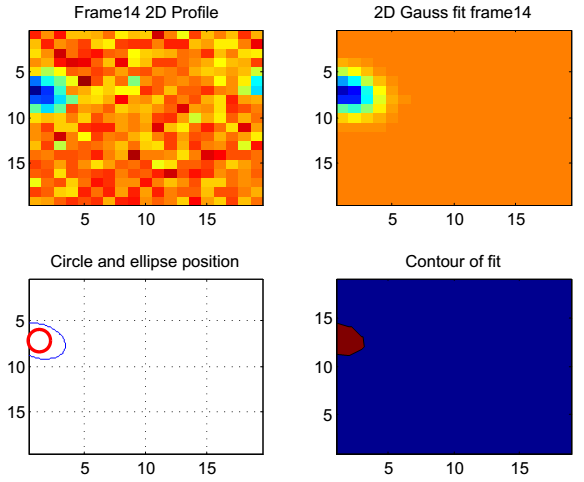
\includegraphics[scale=0.4, natwidth=640, natheight=480]{profile2d_2.png} 	%{h_2.png}	\\
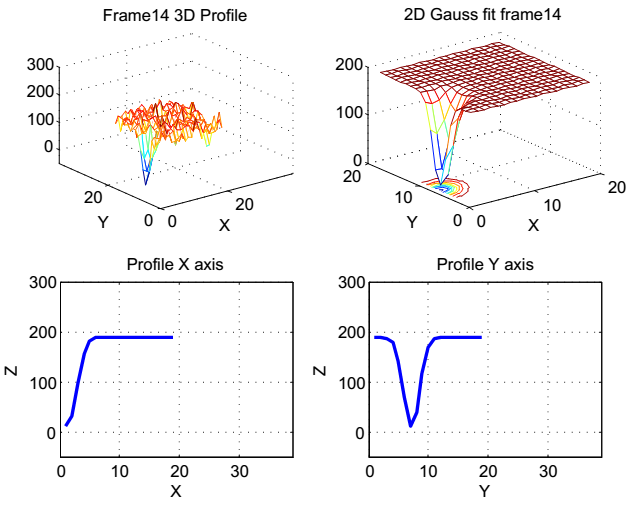
\includegraphics[scale=0.4, natwidth=640, natheight=480]{profile3d_2.png}	%{h_2.png}					
\caption{ Ejemplo de ajuste de gaussian de dos dimensiones a los datos de un frame del STA correspondientes a una unidad cuyo campo receptivo es válido. Izquierda, perfil de dos dimensiones del campo receptivo real (un frame) y su ajuste, mostrando además las elipse respectiva a los parámetros resultantes del ajuste. Derecha, perfiles 3D del frame real y del ajuste gaussiano. }
\label{fig:perfiles1}
\end{figure}
\end{center}

\begin{center}
\begin{figure}[h!]
\centering
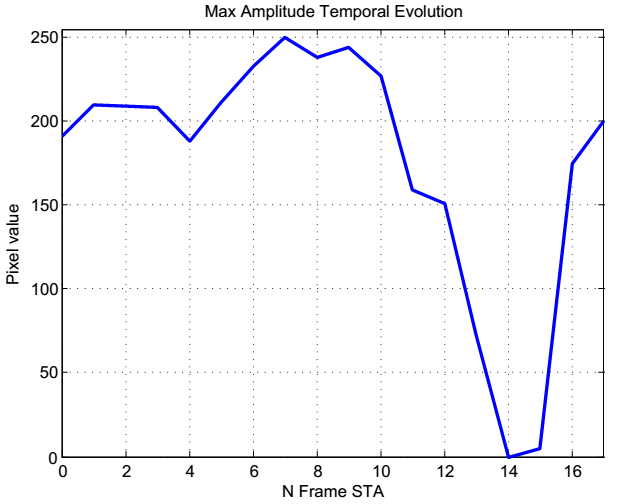
\includegraphics[scale=0.5, natwidth=640, natheight=480]{temporalcurve_2.png} 	%{h_2.png}	\\				
\caption{ Evolución temporal del pixel principal del STA. La posición del pixel principal es elegida de manera que contiene el valor extremo máximo (o mínimo) de todos los pixeles en la matrix STA. }
\label{fig:curvatemporal}
\end{figure}
\end{center}

Las salidas del script corresponden a 4 imágenes (en formato \verb+*.pdf+) y un archivo \verb+*.mat+ con parámetros. La primera imagen corresponde a una vista de todos los frames del STA sin ninguna modificación. La segunda imagen corresponde al perfil 3D del frame de STA original y ajustado, y los perfiles unidimensionales laterales (x, y) del ajuste (ver figura \ref{fig:perfiles1}). La tercera imagen corresponde a los perfiles 2D del frame de STA original y ajustado, y las elipses respectivas (un factor de la desviación estándar en cada eje y el ángulo de la gaussiana). La cuarta imagen corresponde a la curva temporal obtenida (ver figura \ref{fig:curvatemporal}). La curva temporal se construye usando los valores de intensidad de un pixel en particular, en todos los frames del STA. La posición del pixel se elige en base a aquel pixel con el valor extremo máximo (o mínimo) de todos los frames del STA. El archivo \verb+*.mat+ guardado se denomina \verb+fit_var.mat+, y guarda todos los parámetros y datos del frame de STA ajustado.

%=============================================================================
%=============================================================================
%=============================================================================

%%%%%%%%%%%%%%%%% PASTE FIGURE IMAGE EXAMPLE %%%%%%%%%%%%%%%%%%%%%%%%%%%%%%%%%
%\begin{center}
%	\begin{figure}[h!]\label{fig:Esqm}
%			\centering
%			\includegraphics[scale=0.6, natwidth=640, natheight=480]{esquema.png}					
%			\caption{Esquema Problema Planteado}
%		\end{figure}
%\end{center}
%%---------------------------------------------------------------------------%%

%% example of several figures with one caption
%\begin{center}
%	\begin{figure}[h!]\label{fig:h1}
%			\centering
%			\includegraphics[scale=0.3, natwidth=640, natheight=480]{h1.png}	
%			\includegraphics[scale=0.3, natwidth=640, natheight=480]{h22.png}					
%			\caption{Imagen del primer frame de película y región de interés. La región de interés es enmarcada y se muestra la información de intensidad de uno de los canales RGB.}
%		\end{figure}
%\end{center}

%%%%%%%%%%%%%%%%% CITE EXAMPLE %%%%%%%%%%%%%%%%%%%%%%%%%%%%%%%%%%%%%%%%%%%%%
% \nocite{*}
% \bibliographystyle{IEEE}
%%%%%\bibliography{bib-file}  % commented if *.bbl file included, as
%%%%%see below
%%---------------------------------------------------------------------------%%


%%%%%%%%%%%%%%%%% BIBLIOGRAPHY IN THE LaTeX file !!!!! %%%%%%%%%%%%%%%%%%%%%%%%
%% This is nothing else than the IEEEsample.bbl file that you would
%%
%% obtain with BibTeX: you do not need to send around the *.bbl file
%%
%%---------------------------------------------------------------------------%%
\begin{thebibliography}{1}
			 
%	\bibitem{labelreferencia}
%	autor 1, autor2, autor3, 
%	\newblock {\em " titulo titulo titulo"}, 
%	\newblock REVISTA 3 (8) (2009) e3060.			 
		
%	\bibitem{litke2004}
%	A. M. Litke, N. Bezayiff, E. J. Chichilnisky, W. Cunningham, W. Dabrowski, A. A. Grillo, M. Grivich, P. Grybos,
%P. Hottowy, S. Kachiguine, R. S. Kalmar, K. Mathieson, D. Petrusca, M. Rahman, and A. Sher 
%	\newblock {\em " What Does the Eye Tell the Brain: Development of a System for the Large-Scale Recording of Retinal Output Activity"}, 
%	\newblock IEEE TRANSACTIONS ON NUCLEAR SCIENCE, 51 (4) (2004).			

	\bibitem{litke2004} A. M. Litke, N. Bezayiff, E. J. Chichilnisky, W. Cunningham, W. Dabrowski, A. A. Grillo, M. Grivich, P. Grybos,
P. Hottowy, S. Kachiguine, R. S. Kalmar, K. Mathieson, D. Petrusca, M. Rahman, and A. Sher,
	\textit{What Does the Eye Tell the Brain?: Development of a System for the Large-Scale Recording of Retinal Output Activity.}
	IEEE Transactions on Nuclear Science, 51 (4) (2004). 

%	\bibitem{fieldchichilnisky2007}
%	G.D. Field and E.J. Chichilnisky, 
%	\newblock {\em " Information Processing in the Primate Retina:
%Circuitry and Coding"}, 
%	\newblock The Annual Review of Neuroscience. (30) (2007).			 

	\bibitem{fieldchichilnisky2007} G.D. Field and E.J. Chichilnisky,
	\textit{Information Processing in the Primate Retina: Circuitry and Coding.}
	The Annual Review of Neuroscience. (30) (2007).
			 
%	\bibitem{field2007}
%	Greg D. Field, Alexander Sher, Jeffrey L. Gauthier, Martin Greschner, Jonathon Shlens, Alan M. Litke, and E. J. Chichilnisky, 
%	\newblock {\em " Spatial Properties and Functional Organization of Small Bistratified Ganglion Cells in Primate Retina"}, 
%	\newblock The Journal of Neuroscience 27 (48) (2007).			 
			 			 
	\bibitem{field2007} Greg D. Field, Alexander Sher, Jeffrey L. Gauthier, Martin Greschner, Jonathon Shlens, Alan M. Litke, and E. J. Chichilnisky,
	\textit{ Spatial Properties and Functional Organization of Small Bistratified Ganglion Cells in Primate Retina.}
	The Journal of Neuroscience 27 (48) (2007). 
			 
\end{thebibliography}
%%---------------------------------------------------------------------------%%

%=============================================================================

%\noindent \textsc{UTFSM ELO313 2013 - AASTUDILLO}
%\noindent \textsc{ABAC - \today}

%\bibliographystyle{plain}
%\bibliography{c:/0_LaTex/bibliografia}
\end{document}
